\documentclass[10pt]{beamer}

\usetheme[progressbar=frametitle]{metropolis}
\usepackage{appendixnumberbeamer}
\usepackage{pgf}
\usepackage{units}
\usepackage{graphicx}
\usepackage{caption}
\usepackage[mode=buildnew]{standalone}% requires -shell-escape
\usepackage{amsmath}

\usepackage[english]{babel}
\usepackage[utf8x]{inputenc}
\setbeamertemplate{footline}[frame number]

\title{Building an end-to-end speech recognizer}
\author{Moritz Wolter}

\date{01.02.2017}


\begin{document}
\begin{frame}
  \titlepage
\end{frame}


% Uncomment these lines for an automatically generated outline.
\begin{frame}{Outline}
  \tableofcontents
\end{frame}

\section{Worum geht es?}
\begin{frame}{Das Problem}
	\begin{itemize}
		\item Was wird gesagt?
		\item Wie können Text und Ton zugeordnet werden?
		\item Mit welcher Modell-Architektur?
		\item Was sind gute optimierungs-Parameter?
		\item Wie lässt sich gute Generalisierung sicherstellen?
	\end{itemize}
\end{frame}

\begin{frame}{The LAS-Architektur}
	\begin{figure}
		\begin{tikzpicture}
		    \node[anchor=south west,inner sep=0] at (0,0) {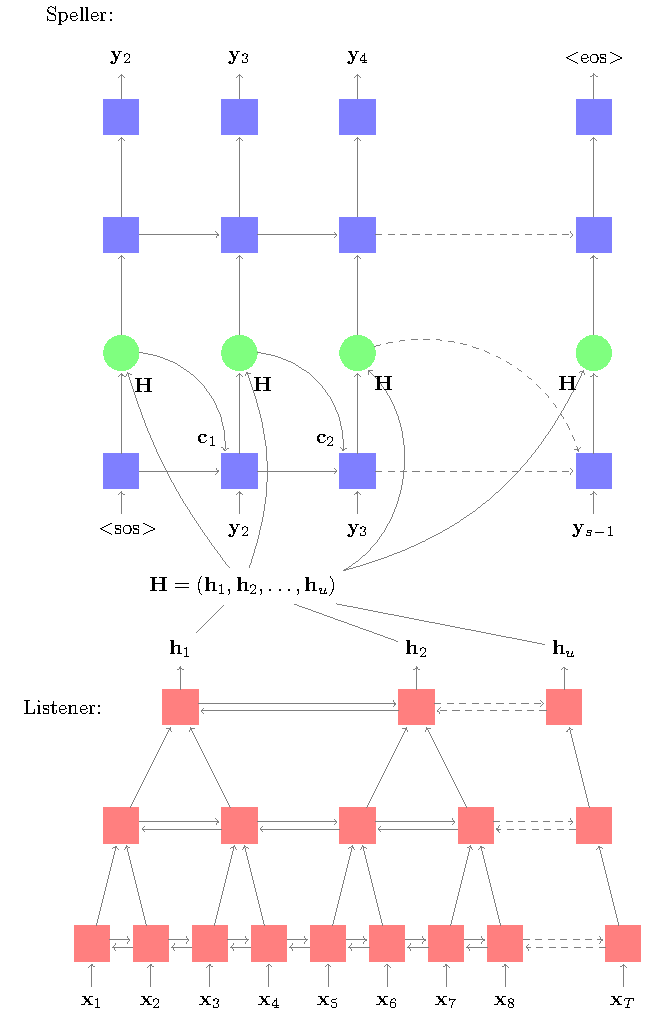
\includegraphics[height=6.5 cm]{../tikz/lasArcBottomUp}};
		    %\draw[red,ultra thick,rounded corners] (0.0,0.0) rectangle (5.0,2.5);
		\end{tikzpicture}
		\caption{Listener und speller.}
	\end{figure}
\end{frame}

\begin{frame}{Die LAS-Gleichungen}
Attend und spell Zell-Berechnungen:
\begin{align}
	 \mathbf{s}_i &= \text{RNN}(\mathbf{s}_{i-1}, \mathbf{y}_{i-1}, \mathbf{c}_{i-1}), \\
	 \mathbf{c}_i &= \text{AttentionContext}(\mathbf{s}_i,\mathbf{H}), \\
	  P(\mathbf{y}_i|\mathbf{x}, \mathbf{y}_{<i}) &= \text{CharacterDistribution}(\mathbf{s}_i,\textbf{c}_i).
\end{align}

AttentionContext Berechnungen:
\begin{align}
	e_{i,u} = \phi(\mathbf{s}_i)^T \psi(\mathbf{h_u}), \\
	\alpha_{i,u} = \frac{ \exp(e_{i,u})}{ \sum\limits_{u} \exp(e_{i,u})}, \\
	\label{eq:alphas}
	\mathbf{c}_i = \sum\limits_{u} \alpha_{i,u} \mathbf{h}_u.
\end{align}
\end{frame}

\section{Implementierung}


\begin{frame}[fragile]
\frametitle{Herausforderungen}
\begin{itemize}

\item Attend und spell Zelle
\item Dekodier-Schliefen-Logik
	\begin{itemize}
	\item Greedy decoding
	\item Beam search
		\begin{itemize}
		\item Mehrere Hypothesen.
		\item Betrachtet die individuelle Wahrscheinlichkeit einzelner
			  Sequenz-Elemente, den Status und die Gesamtlänge.
		\end{itemize}
	\end{itemize}
\item Effizienz
\end{itemize}
\end{frame}

\begin{frame}{Attend und spell Zell Layout}
	\begin{figure}
	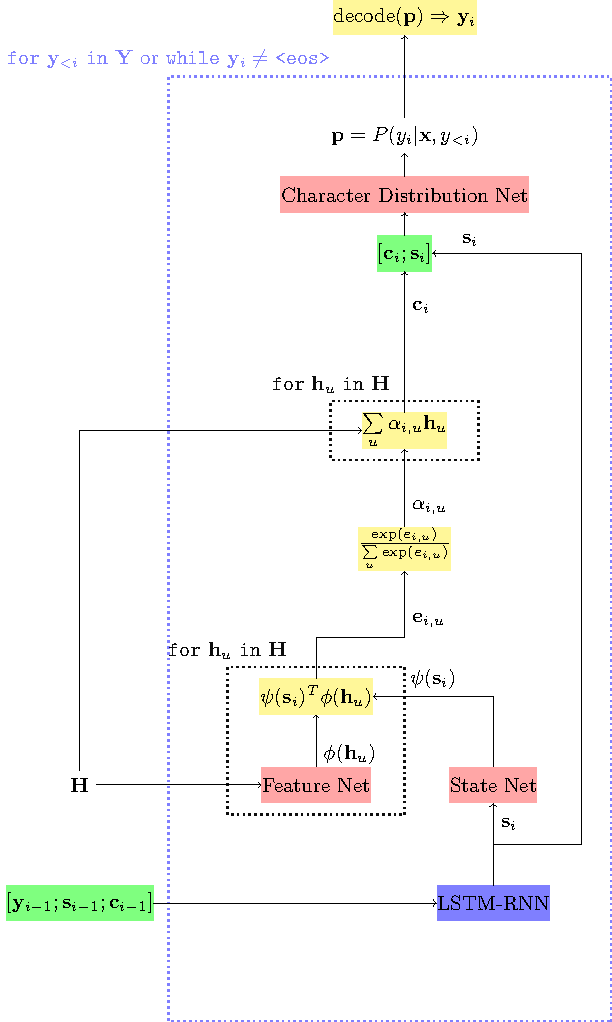
\includegraphics[height=6.5 cm]{../tikz/asCellType1}
	\caption{Attend und spell Zell Flow-Chart.}
	\end{figure}
\end{frame}

\begin{frame}{Effiziente Implementierung}
	\begin{itemize}
		\item Evaluiere das feature Netz außerhalb der Attend und Spell
			  Zelle.
		\item Tensoren mit konstanter Größe für effizienter
			  Speicherallokation.
		\item Sequenzlängen beachten gerade auf dem Sprachsignal.
		\item Sequenzlängen verwenden um keine Nullen zu verarbeiten.
	\end{itemize}
\end{frame}

\begin{frame}{Dropout}
	\begin{figure}
		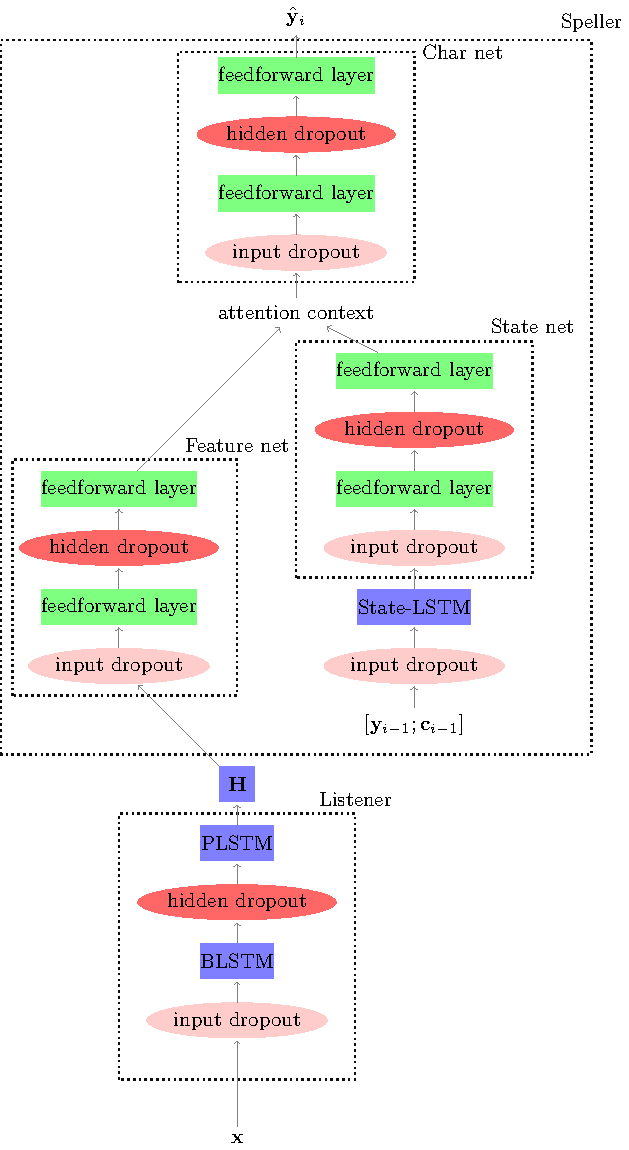
\includegraphics[height=6.5 cm]{../tikz/las_dropout}
		\caption{Input dropout - hellrot. Hidden dropout - dunkelrot.}
	\end{figure}
\end{frame}

\section{Results}

\begin{frame}{Experimental settings}

\begin{itemize}
	\item TIMIT Speech corpus.
	\item Schrittweite: 0.001.
	\item batch\_größe: 16 Sätze, Im Trainings-Datensatz insgesamt 3696.
	\item Validierungsdatensatzgröße: 4 Sätze.
	\item Testdatensatzgröße: 192 Sätze.
	\item Alle 20 schritte ein Validierunsschritt.
\end{itemize}

\end{frame}

\begin{frame}{Aufmerksamkeits plots}
	\begin{figure}
	\centering
	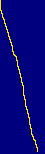
\includegraphics[width=0.2\linewidth, angle=90]{../tikz/align}
	\end{figure}
	\begin{figure}
	\centering
	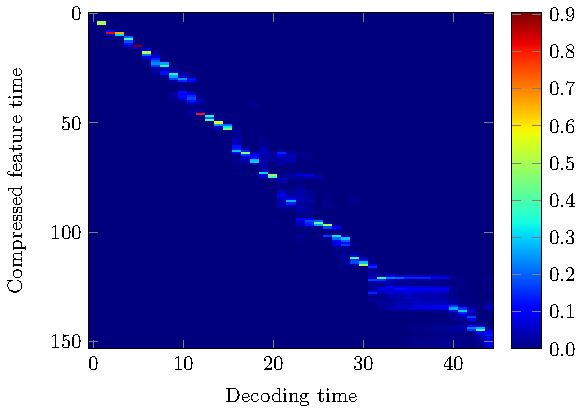
\includegraphics[width=0.2\linewidth, angle=90]{../tikz/alpha}
	\caption{Plot der Aufmerksamkeits Vektoren für alle 45 labels die dem
	Timit sample \texttt{fmld0\_sx295} (unten), zugeordnet wurden und
	Phonemdauer-Zuordnung eines Menschlichen Zuhörers (oben).}
	\label{fig:fullAttention}
	\end{figure}
\end{frame}

\begin{frame}{Aufmerksamkeits plots}
	\begin{block}{Ziel labels}
		\begin{semiverbatim}
		<sos>  sil  ih  f  sil  k  eh  r  l  sil  k  ah  m  z
		       sil  t  ah  m  aa  r  ah  hh  ae  v  er  r  ey
		       n  jh  f  er  m  iy  dx  iy  ng  ih
		       sil  t  uw  sil
		<eos>
		\end{semiverbatim}
	\end{block}

	\begin{figure}
	\centering
	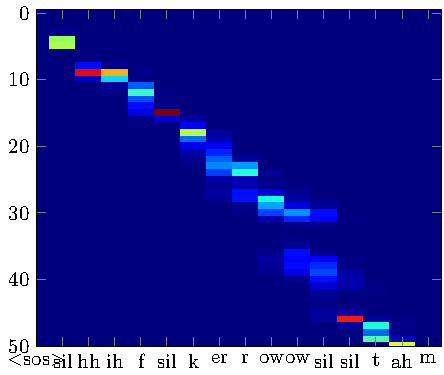
\includegraphics[height=0.26\linewidth]{../tikz/alphaZoom}
	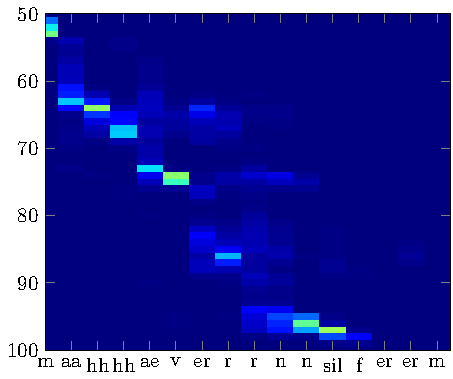
\includegraphics[height=0.26\linewidth]{../tikz/alphaZoom2}
	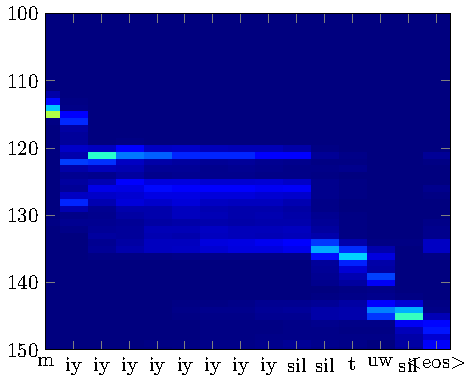
\includegraphics[height=0.26\linewidth]{../tikz/alphaZoom3}
	\caption{Aufmerksamkeits-Gewichte $\alpha$ und Netzwerk output.}
	\label{fig:attention3}
	\end{figure}
\end{frame}

\begin{frame}
	\begin{figure}
	\centering
	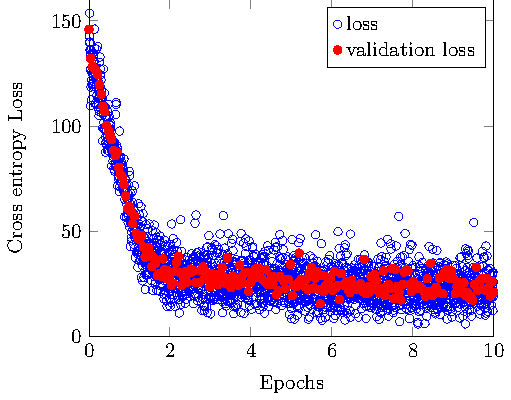
\includegraphics[width=0.24\linewidth]{../tikz/LAS_no_reg_e10_p02_loss}
	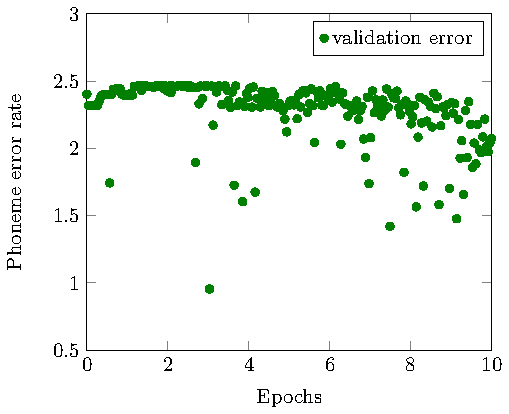
\includegraphics[width=0.24\linewidth]{../tikz/LAS_no_reg_e10_p02_error}
	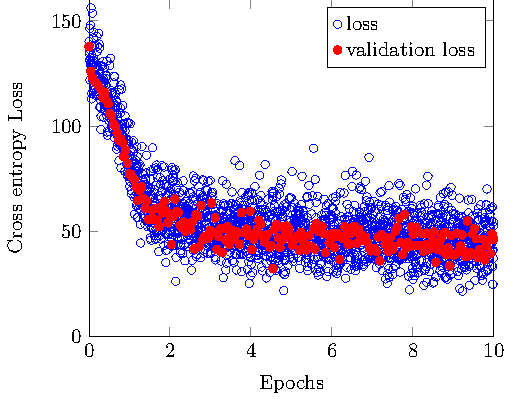
\includegraphics[width=0.24\linewidth]{../tikz/LAS_no_reg_e10_p04_loss}
	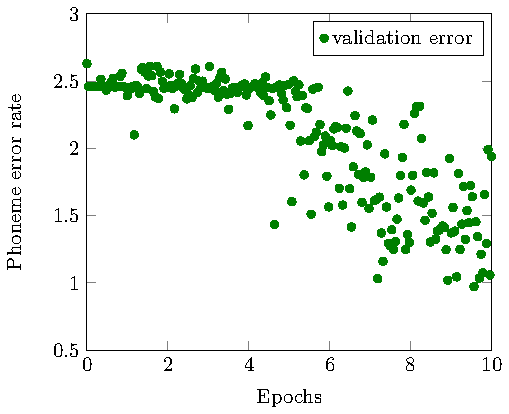
\includegraphics[width=0.24\linewidth]{../tikz/LAS_no_reg_e10_p04_error}
	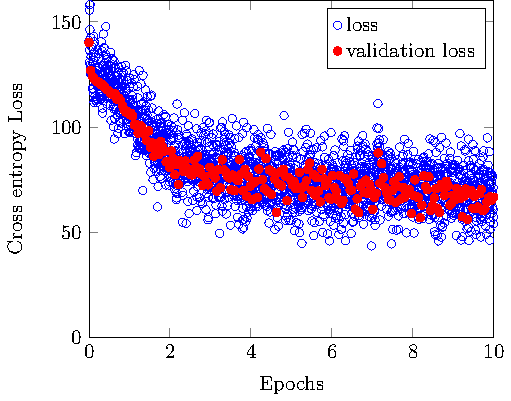
\includegraphics[width=0.24\linewidth]{../tikz/LAS_no_reg_e10_p06_loss}
	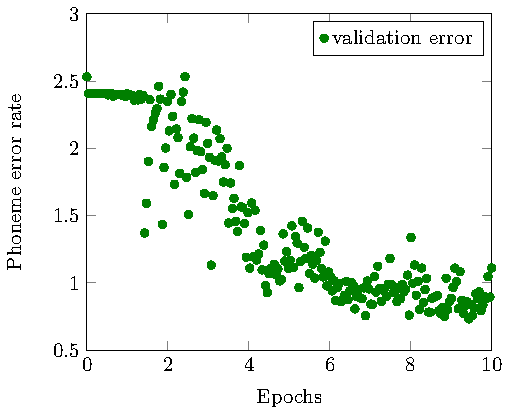
\includegraphics[width=0.24\linewidth]{../tikz/LAS_no_reg_e10_p06_error}
	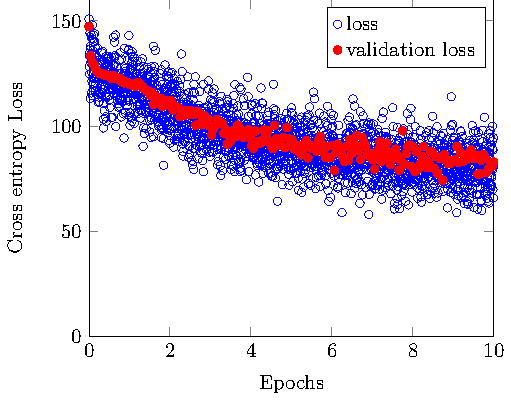
\includegraphics[width=0.24\linewidth]{../tikz/LAS_no_reg_e10_p08_loss}
	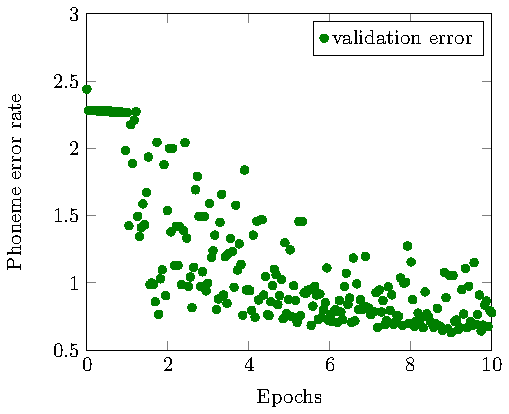
\includegraphics[width=0.24\linewidth]{../tikz/LAS_no_reg_e10_p08_error}
	\caption{Wiederholungen des selben Experimentes mit sich erhöhender
	Rückkopplungs-Wahrscheinlichkeit in der LAS-Zelle $0.2, 0.4, 0.6, 0.8$}
	\label{fig:lasGreedy2468}
	\end{figure}
\end{frame}

\begin{frame}{Dropout las mit beam search}
	\begin{figure}
	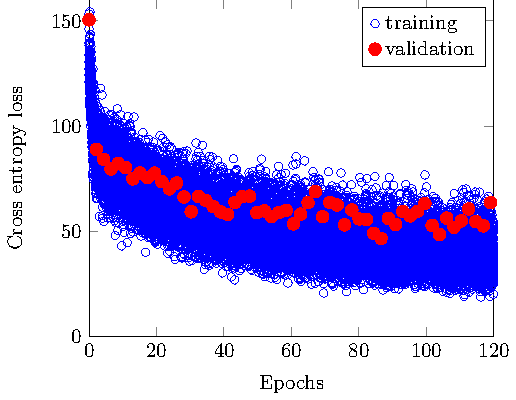
\includegraphics[width=0.49\textwidth]{../tikz/LAS_dropout0805_in00_p06_e120_double_loss}
	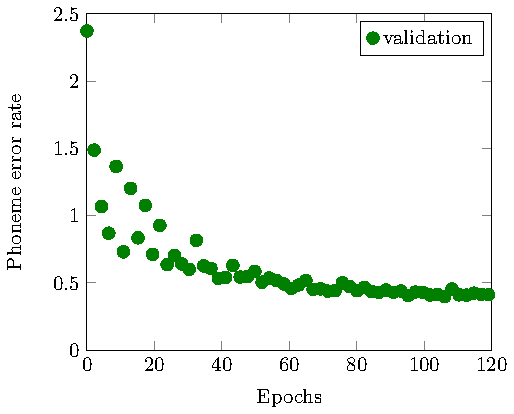
\includegraphics[width=0.49\textwidth]{../tikz/LAS_dropout0805_in00_p06_e120_double_error}
	\caption{Dropout las Ergebnisse.}
	\end{figure}
\end{frame}

\section{Conclusion}
\begin{frame}{Conclusion}

\begin{table}
\adjustbox{max height=\dimexpr\textheight-5.5cm\relax,
           max width=\textwidth}{
\begin{tabular}{ |l c |c c| c c c c| c| r| } \hline
\multicolumn{2}{|c|}{Experiment}  & \multicolumn{2}{|c|}{listener}  & \multicolumn{4}{|c|}{speller}       & epochs & error  \\ \hline
name 		   & 		reg			   	& dim  & layers			   	& dim   & net & layers	& $p$ reuse	  &  	   &        \\ \hline
BLSTM-CTC    & $\sigma_i=.65$          & 64   & 2	  			    & -	  	& -   & -	    & - 		  & 10     & 29\%   \\
Listener-CTC & $\sigma_i=.65$          & 64   & 2	                & -	    & -	  & -	    & -           & 10     & 26.8\% \\ \hline
Greedy-LAS   & $\sigma_i=.65$          & 64   & 2	                & 128   & 64   & 1,2	    & .7         & 40     & 55\%   \\
Greedy-LAS   & $\sigma_i=.65$          & 64   & 2	                & 128   & 64   & 1,2	    & .5         & 40     & 54\%   \\
Big-Beam-LAS   & $p_i=.8$,$p_h=.6$     & 128  & 2	                & 256   & 128  & 1,2	    & .6         & 40     & 45\%   \\ \hline
\end{tabular}
}
\caption{Ausgewählte Parameter und Fehler einiger interessanter Experimente.}
\end{table}

\end{frame}

\begin{frame}{Conclusion}
\begin{itemize}
	\item Keine Erfolge mit re-implementierter LAS-Architektur.
	\item Verbesserungsmöglichkeiten:
		\begin{itemize}
			\item Tensorflow hat mittlerweile einen eigene Aufmerksamkeits
				  Funktionen. .
			\item Mehr Gewichte.
			\item Nutzung eines größeren Datensatzes.
		\end{itemize}
\end{itemize}
\end{frame}


\section{Questions}
\begin{frame}{Questions}
	Thank's for your attention. Questions? \\
	Now, or later \texttt{moritz@wolter.tech}.
\end{frame}


\end{document}
